\chapter{倾向值匹配算法}

\section{引言}

理想情况下,检验策略有效性的黄金标准是基于实验的方法,比如做A/B测试,不同的策略可以随机分配给用户,但是完全随机对照实验存在很多限制,比如成本非常高,操作困难,在实际环境中几乎不可行。而采用非随机对照实验则容易出现组间基线不齐,数据偏倚。

用户被随机分配到策略组和非策略组,这样对效果直接比较是无偏差的。但是,在评估推广微博有效性的实验中,我们几乎没办法将微博用户随机的分配到策略组和非策略组,这种情况下,策略微博和非策略微博被粉丝看到的概率不同,带来的影响力就不同。比如对某项推广策略,采用这个策略发布的微博的演员大多有众多的粉丝,而不采用这项策略的微博的演员粉丝量都较少,那么对于推广效果的评估就会受到演员粉丝量的影响,采用这项策略带来的影响力就会因为发布微博的演员的特性(粉丝量)的干扰而被高估,因此,推广策略和推广效果之间并不是排除了选择偏倚之后的因果关系,而是混淆了用户特性之后的间接关系,如图~\ref{rel}(a)所示。因果分析的目的是建立推广策略和推广效果之间,排除了其他混淆变量的作用后的因果关系,如图~\ref{rel}(b)所示。

\begin{figure}[!htbp]
\centering
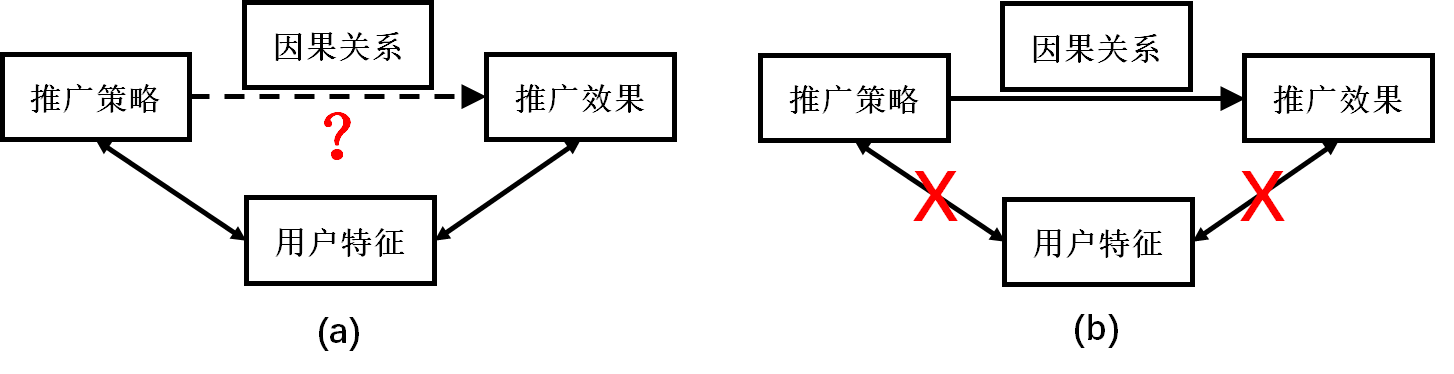
\includegraphics[height=3.5cm]{rel}
\caption{因果关系模型}
\label{rel}
\end{figure}

因此提供一个统计方法而不是实验方法来检测策略的有效性是非常有必要的。最直观地排除用户特性对输出结果影响的方法是建立混淆变量与输出结果之间的回归关系。但是,如果将混淆变量作为自变量放进回归模型,就假定了输出与混淆变量之间存在线性累加关系,这是缺乏依据的,而且,混淆变量与我们研究的策略之间存在一定的相关关系,这样会导致回归模型可能存在共线性问题。

为了解决这个问题,Rosenbaum和Rubin建立了基于观测数据的因果推论模型\cite{rosenbaum1983central},它用倾向值算法作为主要的工具来研究二值策略。将研究对象根据是否采用策略分成策略组和非策略组。其中,倾向值是指在给定混淆变量的基础上,一个研究对象采用该项策略的概率值,通过控制倾向值,可以达到控制混淆变量的目的。对于倾向值的估计,应用最广泛最标准的是Logistic回归模型,也有别的方法可以用来估计倾向值,比如半参回归,无参回归,双重鲁棒估计等等。

倾向值算法被广泛应用在各个领域,包括医药学,经济学,政治学等等,由于其基于观测数据得到的结果更为准确,近几年更是在广告学很受欢迎。

\section{反事实与基本假设}
\subsection{反事实}
设想存在这样一个平行宇宙,演员们在发布推广微博时,除了不使用某项推广策略之外,其他所有条件与现实世界都完全相同。比如还是同样的演员发布同样的微博内容,用来推广同样的电视剧,其他人们事件、热门话题还是依旧发生等等。经过观察,如果在平行宇宙和现实世界,这条推广微博能够达到的推广效果相同,并没有因为使用这项推广策略而改变,那么就可以认为这项推广策略是无效的,它与推广效果之间没有因果关系。这样的平行宇宙假设就叫做反事实,即指相反情境下的某种状态\cite{胡安宁2012倾向值匹配与因果推论}。自变量(推广策略)对于因变量(微博影响力)的因果性效应就是指这些微博在策略组和非策略组能达到的宣传效果之间的差异,也就是事实与反事实之间的差异。

具体来说,定义每一项策略为$t$,作为自变量,其取值为$T$。在二值策略中,$T=\{0,1\}$,其中$T=1$代表采用这项策略,$T=0$代表不采用这项策略。同时,定义达到的效果输出为$Y(T)$,作为因变量。在研究演员推广策略时,用微博影响力作为$Y(T)$。从反事实的框架出发,推广策略的平均干预效果$\Delta$可以利用如下公式来进行衡量:

\begin{equation}
\Delta =\pi\{E[Y(1)|\omega=1]-E[Y(0)|\omega=1]\}+(1-\pi)\{E[Y(1)|\omega=0]-E[Y(0)|\omega=0]\}\\
\label{equ}
\end{equation}

其中$\pi$是分到策略组的微博的比例,那么$1-\pi$就表示分到非策略组的微博的比例。定义$Y$为每条微博达到的推广效果,每条微博都有两个可能的取值,即$Y(0)$和$Y(1)$,$Y(0)$表示如果这条微博没采用该项策略得到的推广效果,$Y(1)$表示如果这条微博采用该项策略得到的推广效果。对于一条微博,因为它只可能采用了或者没采用某项策略,所以$Y(0)$和$Y(1)$的值不可能同时被观测到,其中没被观测到的那个值便是反事实。$E[Y(T)]$表示采用策略$T$的微博的推广效果的期望。$\omega=\{0,1\}$,其中$\omega=1$代表“假设”微博采用了某项策略,$\omega=0$代表“假设”没采用策略。上述公式中,$E(Y(1)|\omega=1)$和$E(Y(0)|\omega=0)$是来自观测数据,对策略的假设与真实情况相符。而$E(Y(1)|\omega=0)$和$E(Y(0)|\omega=1)$则是反事实,分别表示对于采取了策略的微博却“假设”其没采取时所得到的推广效果的期望,和对于没采取策略的微博却“假设”其采取了策略时所得到的推广效果的期望。

\subsection{基本假设}

在因果推论模型中,为了无偏倚的评估策略的效果,通常有两个基本假设:

\textbf{(1)稳定的单位策略输出假设,即观测对象之间没有相互影响。}在一个策略的前提下,对于一个观测对象的潜在输出值应该是稳定的,不受其他观测对象的影响。这个假设使我们能对一个对象的建模不受其他对象的影响。

\textbf{(2)强忽略假设,即非混淆假设。}在给定混淆变量的条件下,策略是否采用与输出结果独立。这个假设使我们能在混淆变量给定时,对是否采用策略进行建模时,与输出结果无关。具体地,非混淆假设是指满足:

\begin{equation}
\begin{cases}
E(Y(1)|\omega=0)=E(Y(1)|\omega=1)\\
E(Y(0)|\omega=0)=E(Y(0)|\omega=1)
\end{cases}
\end{equation}

根据非混淆假定,将其带入公式~\ref{equ}可以得到推广策略的平均干预效果为:

\begin{equation}
\Delta=E[Y(1)|\omega=1]-E[Y(0)|\omega=0]
\end{equation}

\section{倾向值匹配算法步骤}

在倾向值匹配算法中,混淆变量是指可能与自变量和因变量有一定相关性,而干扰自变量与因变量之间的因果关系的变量。如演员A和演员B发布的微博带来的影响力的不同,除了策略的不同,还可能是因为二者的粉丝量不同带来的差异。这些混淆变量对推广效果的影响就是选择性误差,在倾向值匹配算法中,通过控制混淆变量来遏制选择性误差对结果的影响,对混淆变量的控制是通过将混淆变量纳入概率模型(如Logistic回归模型),得到倾向值$P$来进行控制。

定义混淆变量为向量$X$。那么对每一个研究对象$i=1,2, ...,N$,都有混淆变量向量$X_i$,策略$t_i$,输出结果$Y_i$。

\subsection{计算倾向值}

倾向值是指在可观测到的混淆变量的基础上,一个研究对象采用该项策略的条件概率,定义为:
\begin{equation}
e_i = Pr(T_i = 1 | X_i)
\end{equation}
倾向值是一种平衡值,通过控制倾向值可以控制混淆变量,进而使策略组和非策略组的混淆变量类似。对倾向值的估计,本文采用的是逻辑斯地回归模型,建立混淆变量的回归关系,公式如下,训练得到参数进而得到Logistic回归模型,之后便可以计算采用策略的概率值。

\begin{equation}
e_i = Pr(T_i=1|X_i;\theta)=g(z)=\frac{1}{1+e^{-z}}
\end{equation}
其中$\theta$为参数,$z=\theta^Tx=\theta_0+\theta_1X_{i1}+\theta_2X_{i2}+...+\theta_jX_{ij}$,$X_{ij}$表示研究对象$i$的混淆变量的第$j$个分量。

除了最常用的Logistic回归模型,还有装袋法、递归分割法、基于树的方法、半参回归、无参回归、双重鲁棒估计和神经网络等方法都可以用于估计倾向值。

\subsection{倾向值匹配}

根据是否采用了策略,整个样本集合可以分成两个子集合:策略组和非策略组。倾向值匹配意味着对策略组和非策略组中有相似倾向值的样本进行配对,最常用的配对方法是一对一配对,就是说一个策略组的对象可以与一个非策略组的对象配对。还可以一对多匹配($1:M$),多对一($M:1$)匹配,多对多($M:M$)匹配等。在匹配算法的选取上,首先,要选择用可替换还是不可替换的算法。不可替换算法意味着一旦一个非策略组的对象与一个给定的策略组的对象匹配后,就不可以再与其他策略组的对象进行匹配。因此,每个非策略组的对象只能最多被一个匹配对儿包含。与之对比,可替换算法中,非策略组的对象还可以与策略组的其他对象进行匹配,所以非策略组的对象可能被多个匹配对儿包含。然后,要选择用贪心匹配还是优化匹配。贪心匹配算法中,先从策略组中随机选一个对象,然后从非策略组中选取与之倾向值最接近的对象,一直重复直到所有的策略组或者非策略组的对象都已配对。这个过程中,每一步都是贪心选择非策略组中最接近的对象,而不管这个对象是否与下一个策略组中选中的对象更接近。在优化匹配算法中,配对原则是最小化所有匹配的对儿之间的倾向值差异。

最后,对距离最接近的标准有最邻近匹配和基于卡尺的最近邻匹配。最邻近匹配是指对给定的策略组的对象,选取非策略组中与之倾向值最接近的对象。基于卡尺的最近邻匹配与之相似,只是会多一个卡尺的限制,倾向值的差异在一个卡尺的范围内,匹配最近邻的对象。那么,如果一个策略组的对象在卡尺的范围内没有非策略组的对象,这个策略组的对象就匹配不到。经过研究,奥斯汀\cite{austin2011optimal}发现最佳的卡尺宽度是倾向值对数的标准差的$0.2$倍,这个距离被证明在多种参数设置中会产生最优的风险差异估计。

在本文中,我们应用的是可替换的一对多匹配,距离标准用基于卡尺的最近邻匹配原则,卡尺宽度为倾向值对数的标准差的$0.2$倍。

\subsection{评估策略效果并检验显著性}

在基于倾向值对样本进行匹配后,就可以通过配对后的样本的输出$Y(T)$的差异来估计策略效果。如果输出是连续值,则策略效果可以由策略组和非策略组的输出结果的平均值的差值得到;如果输出是二值的,则策略效果可以由比较策略组和非策略组的二值比例的差异或者相对风险得到。平均干预效果(Average Treatment Effect,ATE)定义如下,它是定义在整个对象集合的基础上的平均效果。

\begin{equation}
ATE = E[Y(1)|\omega=1] - E[Y(0)|\omega=0]
\end{equation}

另一个相似的定义是最终接受策略对象的平均干预效果(Average Treatment effect for the Treated, ATT),它是定义在最终接受了策略的对象基础上的平均干预效果。

\begin{equation}
ATT = E[Y(1) - Y(0) | \omega= 1]
\end{equation}

需要根据研究的需求来进行二者的选择,比如,在评估系统参与到戒烟项目中导致
戒烟成功的有效性时应该用ATT,因为不可能所有的人都参与到具体戒烟项目中;而在评估给家庭发戒烟相关小册子导致戒烟成功的有效性时应该用ATE,因为给每个家庭发戒烟相关小册子的成本相对低、易实现。由于本文中研究的对象是最终用了某项策略的微博,因此我们选用ATT来评估平均干预效果。

之后,需要用t检验(t-test)来检验干预效果的显著性水平,即检验策略组和非策略组配对的样本的效果输出$Y(T)$是否有显著差异,我们将策略组和非策略组配对的样本的输出数据输入到统计软件SPSS中进行t检验。

\subsection{平衡性诊断}

平衡性检验能评估倾向值模型是否经过了充分的验证。倾向值匹配是通过匹配近似的倾向值来达到控制混淆变量类似的目的,因此检验配对样本在混淆变量上是否有显著差异是必不可少的,它代表了配对的样本在混淆变量上的相似程度。标准化均数差能用于量化策略组和非策略组的样本的混淆变量在平均值上的差异。对连续混淆变量,其标准化均数差为:

\begin{equation}
d = \frac{(\overline{x}_{treated} - \overline{x}_{untreated})}{\sqrt{\frac{s_{treated}^2 + s_{untreated}^2}{2}}}
\end{equation}

其中,$\overline{x}_{treated}$和$\overline{x}_{untreated}$分别对应策略组和非策略组样本的连续混淆变量的均值, $s_{treated}^2$和$s_{untreated}^2$分别对应策略组和非策略组样本的连续混淆变量的方差。对二值混淆变量,其标准化均数差为:

\begin{equation}d = \frac{(\hat{p}_{treated} - \hat{p}_{untreated})}{\sqrt{\frac{\hat{p}_{treated}(1 - \hat{p}_{treated}) + \hat{p}_{untreated}(1 - \hat{p}_{untreated})}{2}}}\end{equation}

其中,$\hat{p}_{treated}$和$\hat{p}_{untreated}$分别对应策略组和非策略组样本的二值混淆变量的均值。通常认为,标准均数差数值小于$0.1$时认为配对的策略组和非策略组的样本的混淆变量很类似,达到平衡的状态\cite{normand2001validating}。但是,标准化均数差只是比较了平均值是否类似,还应该比较配对的策略组和非策略组的样本的混淆变量的整体分布是否类似。可以用图形化方法如并列箱形图,分位数-分位数图(Q-Q图),累积分布图等等。

本文用标准化均数差来比较配对样本的混淆变量平均值上的差异,然后用累计分布图和Q-Q图来看配对的样本的混淆变量的分布是否一致。

\section{本章小结}

本章主要对倾向值匹配算法进行了简要介绍。通过对事实与反事实之间的比较来衡量推广策略的推广效果,并根据实际应用情况介绍了倾向值匹配算法的计算步骤,包括利用Logistic回归模型计算倾向值,利用算法进行倾向值匹配,根据匹配结果评估策略效果,并进行显著性检和平衡性诊断。在下一章将该算法应用在演员发布的推广微博上,分析不同的推广策略同推广效果之间的因果关系,从而选取最优的推广策略。






















